% !TeX spellcheck = cs_CZ
%{\tikzset{external/prefix={tikz/FYZII/}}
% \tikzset{external/figure name/.add={ch15_}{}}
%---------------------------------------------------------------------------------------------------
% file fey2ch15.tex
%---------------------------------------------------------------------------------------------------
%=========================== Kapitola: Vektorový potenciál =========================================
\setchaptertoc
\chapter{Vektorový potenciál}\label{fyz:IIchapXV}

  \section{Síly působící na proudovou smyčku. Energie dipólu}\label{fyz:IIchapXVsecI}
    V předcházející kapitole jsme zkoumali magnetické pole vytvořené malou proudovou smyč­kou.
    Zjistili jsme, že jde o dipólové pole s dipólovým momentem
    \begin{equation}\label{fyz:eq585}
      \mu = I S,
    \end{equation}
    přičemž \(I\) je proud a \(S\) je plocha smyčky. Směr momentu je kolmý na rovinu smyčky, a proto
    můžeme psát
    \begin{equation}\label{fyz:eq586}
      \vec{\mu} = I S\vec{n},
    \end{equation}
    kde \(\vec{n}\) je jednotkový vektor normály k ploše \(S\).

    Proudová smyčka - nebo magnetický dipól - nejen že vytváří magnetické pole, ale je zároveň
    vystaven působení sil, je-li vložen do magnetického pole jiných proudů. Nejdříve si všimneme
    síly působící na pravoúhlou smyčku v homogenním magnetickém poli. Nechť osa \(z\) směřuje podél
    pole a osa \(y\) leží v rovině smyčky, která s rovinou \(xy\) svírá úhel \(\vartheta\) (obr.
    \ref{fyz:fig663}). 

  \section{Mechanická a elektrická energie}\label{fyz:IIchapXVsecII}
  \section{Energie ustálených proudů}\label{fyz:IIchapXVsecIII}
  \section{B nebo A}\label{fyz:IIchapXVsecIV}
  \section{Vektorový potenciál a kvantová mechanika}\label{fyz:IIchapXVsecV}
  \section{Co platí ve statice neplatí v dynamice}\label{fyz:IIchapXVsecVI}
  \section{Příklady a cvičení}\label{fyz:IIchapXVsecVII}

    \begin{figure}[ht!] %\ref{fyz:fig663}
      \centering
      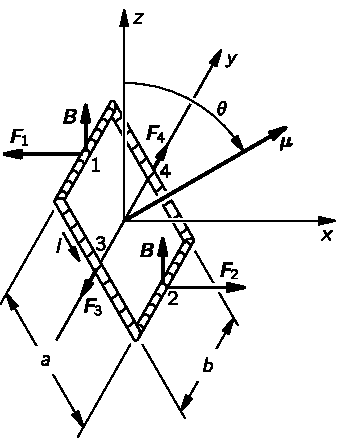
\includegraphics[width=0.7\linewidth]{fyz_fig663.pdf}
      \caption{
               (\cite[s.~707]{Feynman02})}
      \label{fyz:fig663}
    \end{figure}

    \begin{figure}[ht!] %\ref{fyz:fig664}
      \centering
      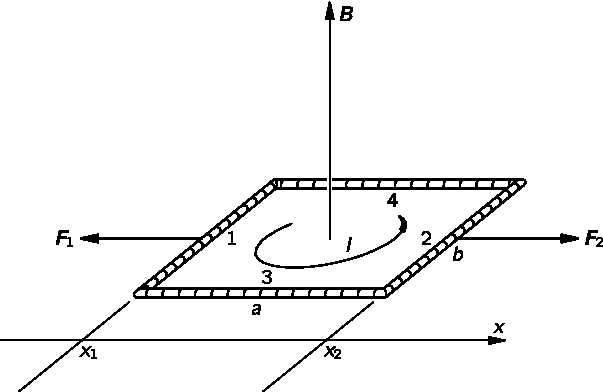
\includegraphics[width=0.7\linewidth]{fyz_fig664.pdf}
      \caption{
               (\cite[s.~707]{Feynman02})}
      \label{fyz:fig664}
    \end{figure}

    \begin{figure}[ht!]
      \centering
      \subcaptionbox{\label{fyz:fig665a}}{\luafigure[0.9]{fyz_fig665a.pdf}}               \\
      \subcaptionbox{\label{fyz:fig665b}}{\luafigure[0.9]{fyz_fig665b.pdf}}
      \label{fyz:fig665}
      \caption{
               (\cite[s.~748]{Feynman02})}
    \end{figure}

    \begin{figure}[ht!] %\ref{fyz:fig666}
      \centering
      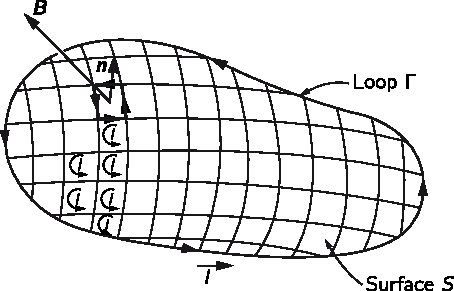
\includegraphics[width=0.7\linewidth]{fyz_fig666.pdf}
      \caption{
               (\cite[s.~707]{Feynman02})}
      \label{fyz:fig666}
    \end{figure}

    \begin{figure}[ht!] %\ref{fyz:fig667}
      \centering
      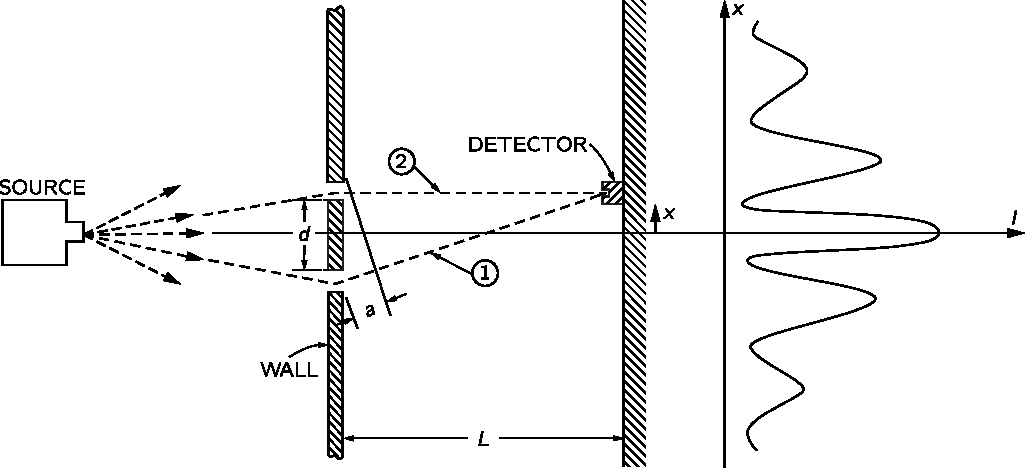
\includegraphics[width=0.7\linewidth]{fyz_fig667.pdf}
      \caption{
               (\cite[s.~707]{Feynman02})}
      \label{fyz:fig667}
    \end{figure}


    \begin{figure}[ht!] %\ref{fyz:fig668}
      \centering
      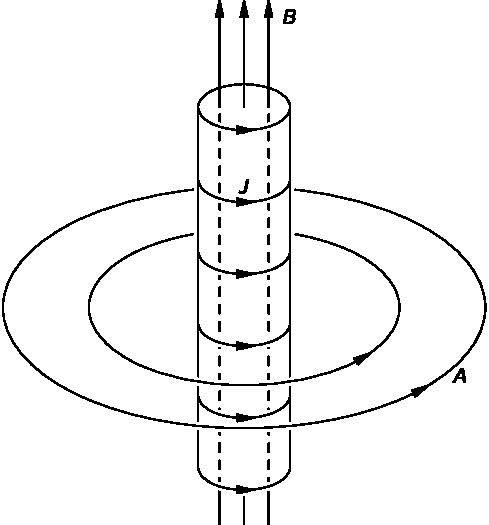
\includegraphics[width=0.7\linewidth]{fyz_fig668.pdf}
      \caption{
               (\cite[s.~707]{Feynman02})}
      \label{fyz:fig668}
    \end{figure}

    \begin{figure}[ht!] %\ref{fyz:fig669}
      \centering
      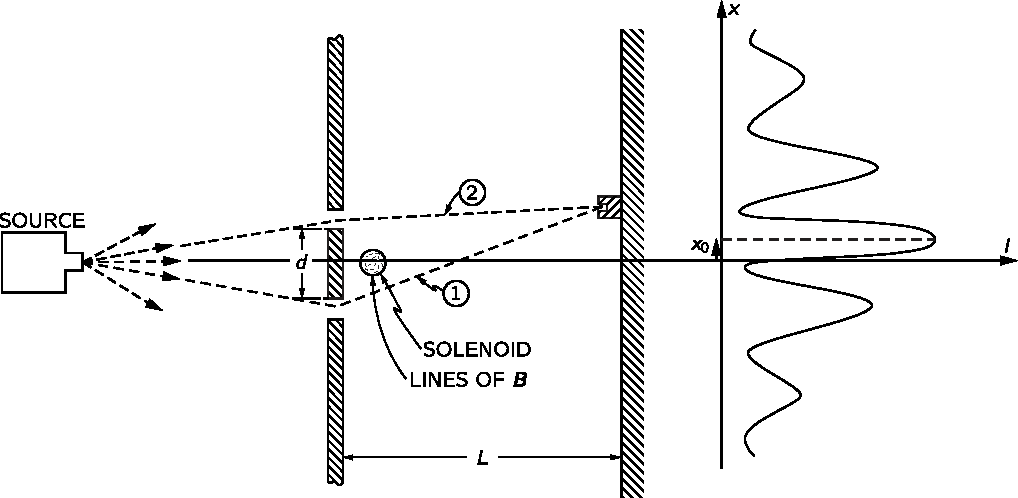
\includegraphics[width=0.7\linewidth]{fyz_fig669.pdf}
      \caption{
               (\cite[s.~707]{Feynman02})}
      \label{fyz:fig669}
    \end{figure}

    \begin{figure}[ht!] %\ref{fyz:fig670}
      \centering
      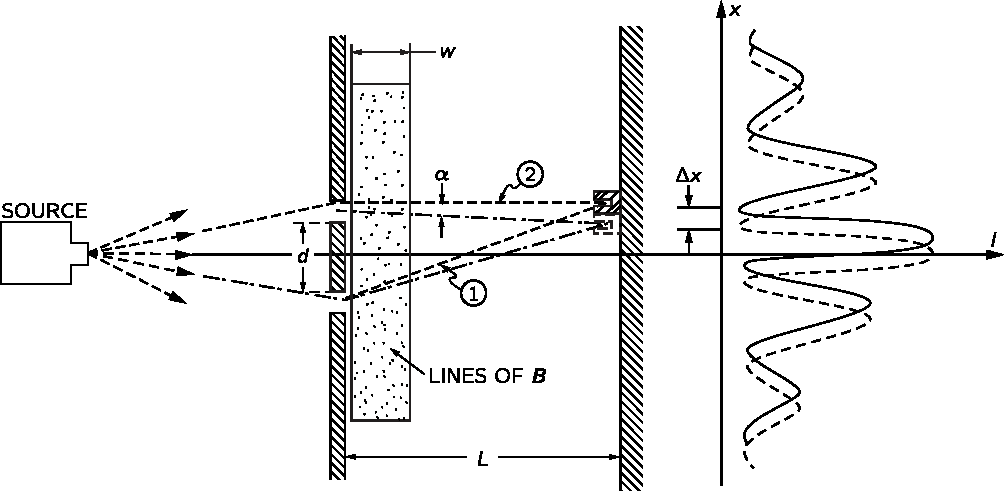
\includegraphics[width=0.7\linewidth]{fyz_fig670.pdf}
      \caption{
               (\cite[s.~707]{Feynman02})}
      \label{fyz:fig670}
    \end{figure}


    \begin{figure}[ht!] %\ref{fyz:fig671}
      \centering
      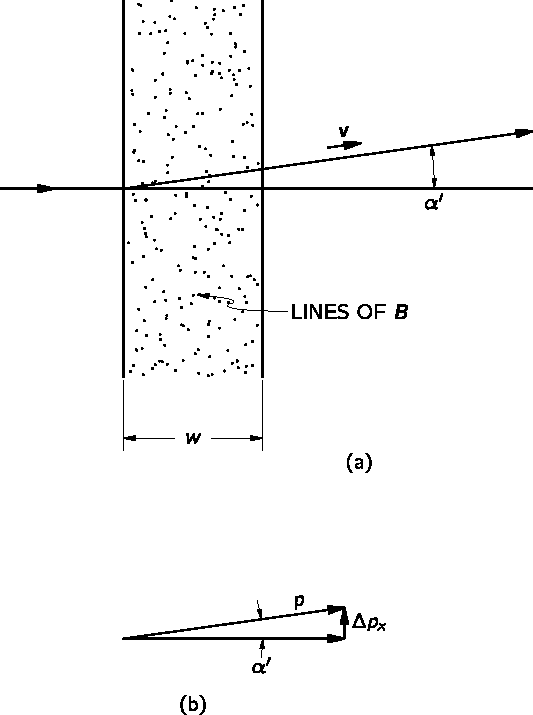
\includegraphics[width=0.7\linewidth]{fyz_fig671.pdf}
      \caption{
               (\cite[s.~707]{Feynman02})}
      \label{fyz:fig671}
    \end{figure}

    \begin{figure}[ht!] %\ref{fyz:fig672}
      \centering
      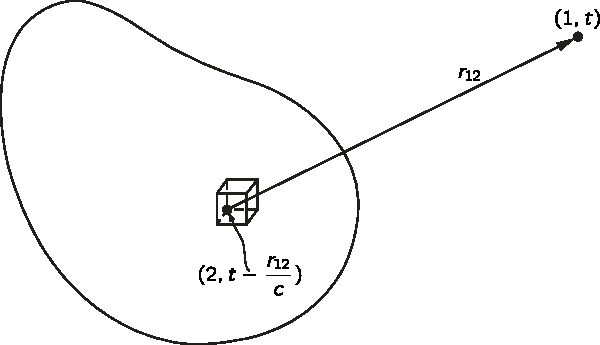
\includegraphics[width=0.7\linewidth]{fyz_fig672.pdf}
      \caption{
               (\cite[s.~707]{Feynman02})}
      \label{fyz:fig672}
    \end{figure}

    \todo[inline]{Kapitola fey2ch15 je nedodělaná, obsahuje pouze obrázky}
%} %tikzset
%---------------------------------------------------------------------------------------------------
